%!TEX root = ../main.tex
\subsection{Implementing CAN utilizing XCanPs}\label{sec:methods_to_implement_can}

\mikkel{DONE:move axi can to analysis.}
\mikkel{move assymetric multiprocesssing to future work}
\mikkel{ move bare metal first}
\mikkel{split from linux part.}

\martin{The can controllers do not have anything to do with xilinux. Does Xilinux provide drivers for the can controllers on the zynq? CAN controllers vs CAN drivers Issue - Some things rephrased.}
After testing the stack board and showing the basic functionality of the CAN network as described in section \ref{sub:TestingCANStack_BareMetal}, the next step was to implement it using Linux running on the Zybo board.\\
Using Linux was necessary because the available sensors, GPS and IMU, as well as the WiFi dongle required an USB interface and the WiFi node needed various networking tools only present on a Linux operating system.
The process of establishing a wireless communication is explained in section \ref{sec:wifi}.
An operating system was also required for logging purposes, specifically to log data into files.
This section describes the necessary procedures that were followed in order to gain control over the CAN network from Linux.
~\\
At this point the reader should be informed that although the CAN controllers could be used on the Processing System using bare-metal code, the implementation of CAN on the Programmable Logic and the access to it from Linux was not successful.
Alternatively, other means to prove the concept of the project were taken into account, as described in section \ref{sub:Utilizing_Svr_Virtualization}.

\subsubsection*{Enabling the CAN Controller Drivers}

This was the first idea on how to utilize the CAN network using Linux.
In order to gain access to the CAN controllers on the Zynq7 Processing System, the Linux CAN driver guide \cite{Xilinx_wiki_Linux_CAN_driver} was followed in order to enable the necessary drivers.
The Kconfig file under the path \ref{code:can_kconfig_pathfile} needed to be configured.
The entry at line 128 was changed as seen in the code snippet \ref{code:can_kconfig_contents_line128}.
Originally, lines 130 and 131 were as seen in the snippet \ref{code:can_kconfig_original_line130}.

\begin{lstlisting}[caption={CAN Kconfig pathfile.},numbers=none,label=code:can_kconfig_pathfile]
/usr/src/kernels/3.12.0-xillinux-1.3/drivers/net/can
\end{lstlisting}

\begin{lstlisting}[firstnumber=128,caption={Kconfig file contents from line 128.},label={code:can_kconfig_contents_line128}]
config CAN_XILINXCAN
	tristate "Xilinx(*@ @*)CAN"
	depends on NET [=y] && CAN_DEV [=y] && CAN [=y] && 
        (ARCH_ZYNQ || MICROBLAZE [=y])
	default y
\end{lstlisting}

\begin{lstlisting}[firstnumber=130,caption={Original content of lines 130 and 131.},label={code:can_kconfig_original_line130}]
	depends on CAN && (ARCH_ZYNQ || MICROBLAZE)
	default n
\end{lstlisting}

The next step of the process was the modification of the device tree settings file, requiring an entry for the CAN PS to be inserted.
The necessary file was located under the boot folder named as seen in \ref{code:dts_file_zybo}.
The modifications can be seen in the snippet \ref{code:dts_changes_zybo} for can controllers as well as for the AXI CAN core.

\begin{lstlisting}[numbers=none,caption={Device tree settings file and its path.},label={code:dts_file_zybo}]
/boot/xillinux-1.3-zybo.dts
\end{lstlisting}
\catalin{Double quotes are problem here as well. FIX THEM WHENEVER}
\begin{lstlisting}[caption={Device tree settings changes.},label={code:dts_changes_zybo}]
zynq_can_0: can@e0008000 {
        compatible = xlnx,zynq-can-1.0;
        clocks = <&clkc 19>, <&clkc 36>;
        clock-names = can_clk, pclk;
        reg = <0xe0008000 0x1000>;
        interrupts = <0 28 4>;
        interrupt-parent = <&intc>;
        tx-fifo-depth = <0x40>;
        rx-fifo-depth = <0x40>;
    };
axi_can_0: axi-can@40000000 {
        compatible = xlnx,axi-can-1.00.a;
        clocks = <&clkc 0>, <&clkc 1>;
        clock-names = can_clk,s_axi_aclk;
        reg = <0x40000000 0x10000>;
        interrupt-parent = <&intc>;
        interrupts = <0 59 1>;
        tx-fifo-depth = <0x40>;
        rx-fifo-depth = <0x40>;
        };
\end{lstlisting}

\mikkel{Maybe you can provide some thoughts about the problem. Maybe also some words about the patching Xilinx-Digilent etc.}
As was previously mentioned, the implementation was unsuccessful. At the time, the research done on this topic did not lead to successfully enabling the drivers.

%The architecture can be seen in figure \ref{fig:CAN_Arch_with_AXI_CAN}.

%\begin{figure}[h!]
%	\centering
%	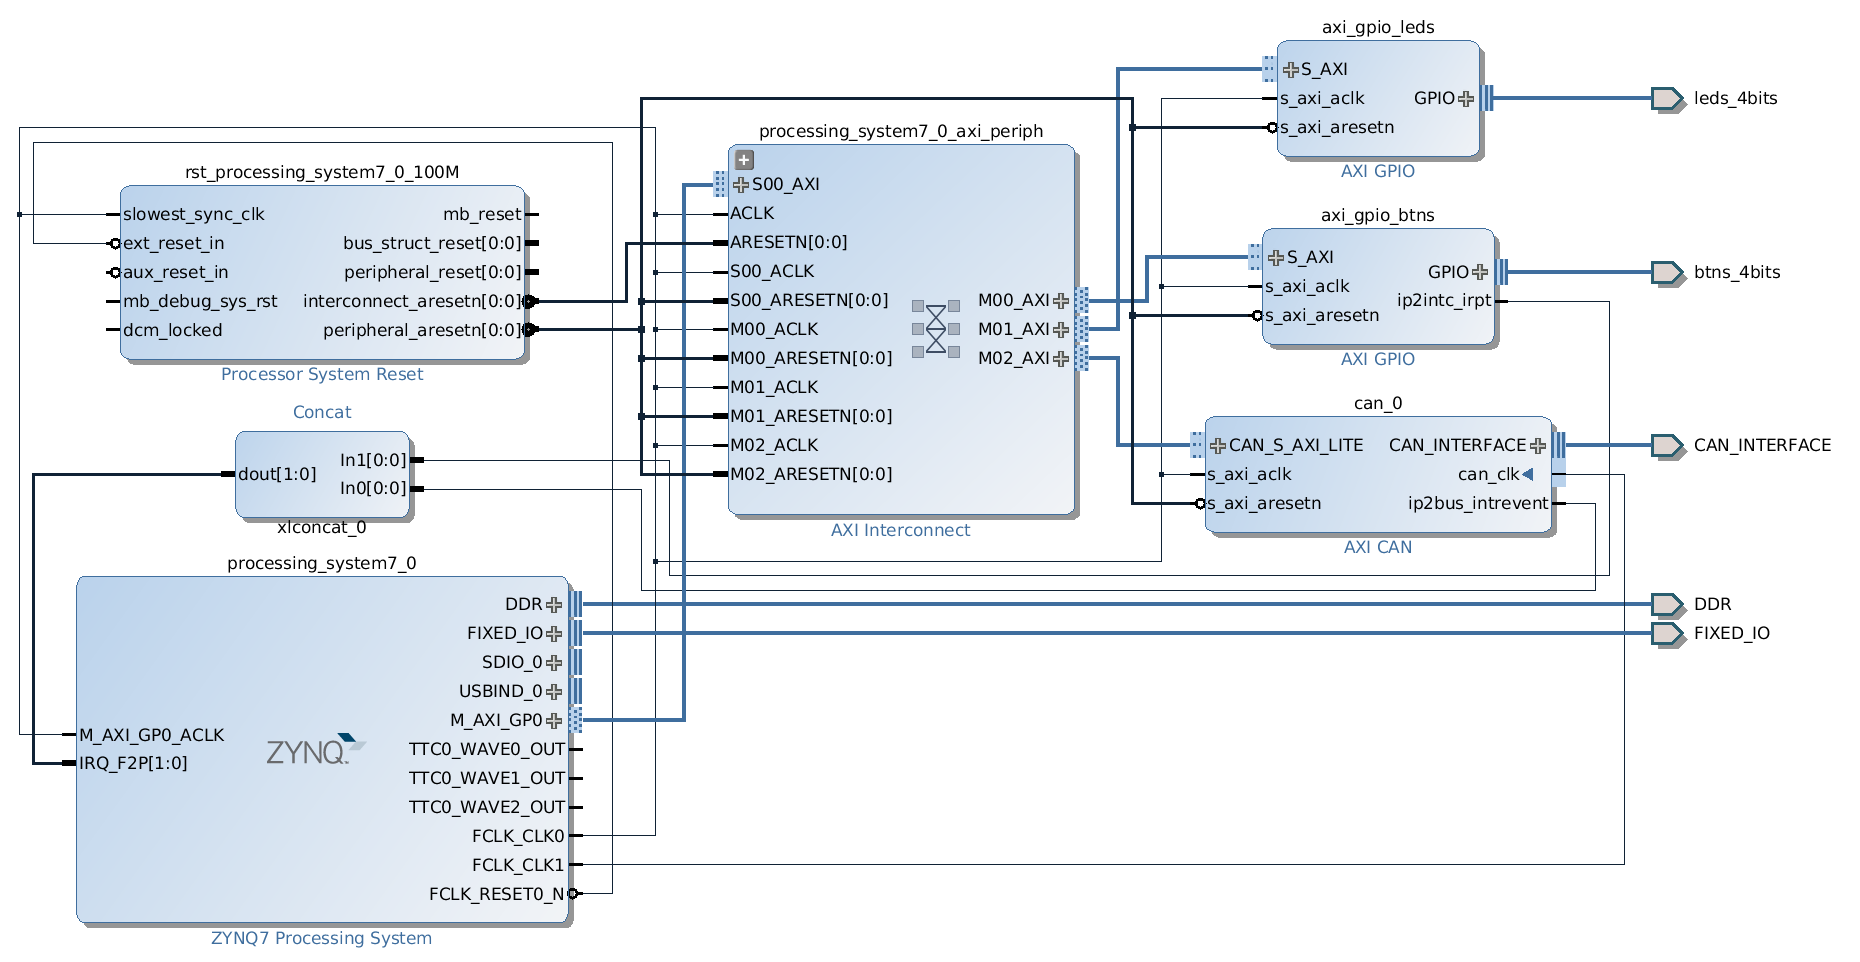
\includegraphics[width = 1.2\linewidth]{graphics/Zybo_Arch_with_AXI_CAN.png}
%	\caption{Block diagram featuring the architecture in Vivado with the AXI CAN core.}
%	\label{fig:CAN_Arch_with_AXI_CAN}
%\end{figure}
